% Merkhilfe SQL zum Notebook sql_abfragen (https://ktheu.github.io/python-uebungen/)
% Übersetzen (im Ordner merkhilfen):  latexmk -pdf sql.tex
% Das Schema-Bild kino_schema.png erzeugt:  py -3.13 merkhilfen/kino_schema.py
\documentclass[9pt,a4paper,landscape]{extarticle}
\usepackage{merkhilfe}
\lstset{basicstyle=\ttfamily\small}

\begin{document}
\merktitel{Merkhilfe SQL}{Notebook sql\_abfragen \quad ktheu.github.io/python-uebungen}

\begin{center}
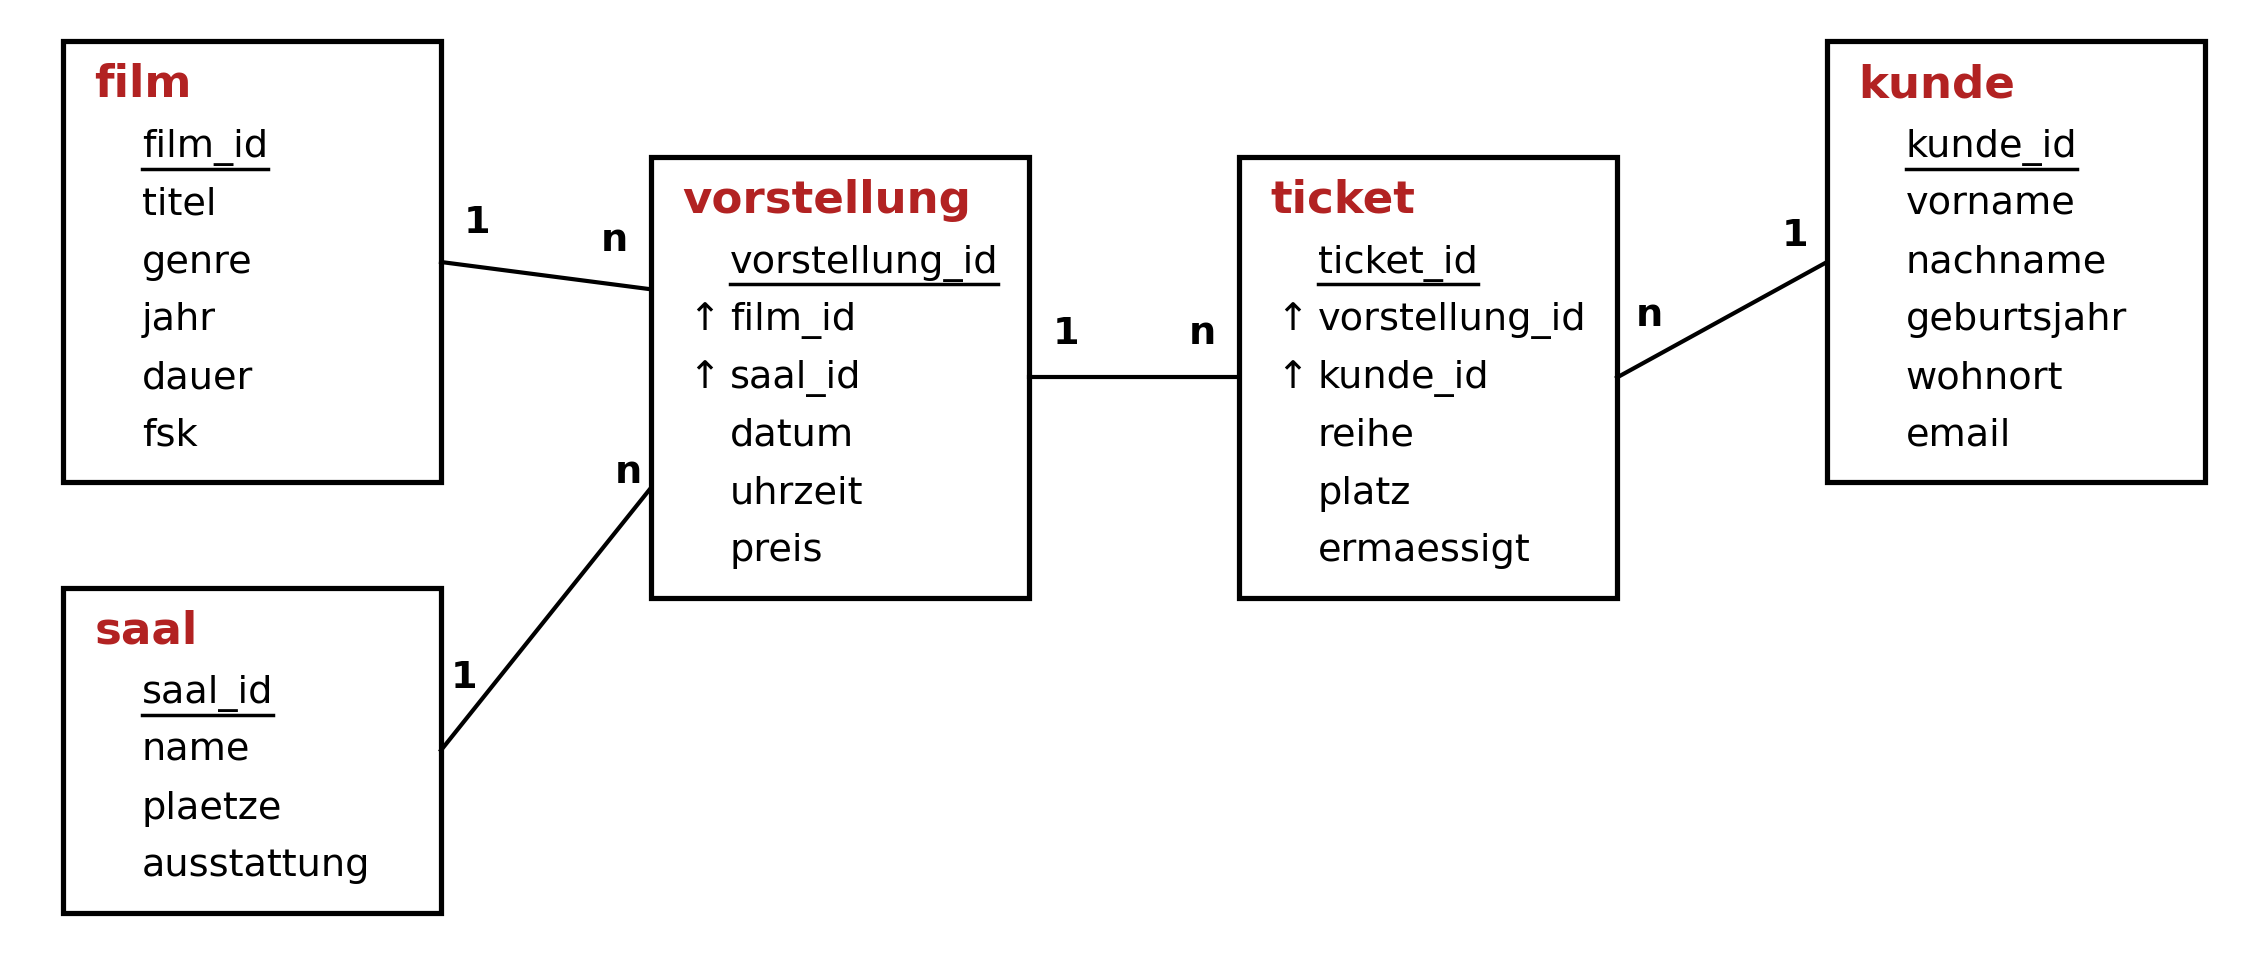
\includegraphics[height=5.3cm]{kino_schema.png}\par
{\footnotesize\color{grau}Datenbank \texttt{kino.db}: Primärschlüssel unterstrichen, $\uparrow$ Fremdschlüssel, Linien mit 1 und n}
\end{center}
\vspace{-2pt}

\begin{multicols*}{3}
\begin{merkblock}{Start}{}
\lstinline@%LOAD kino.db r@\st{Datenbank öffnen}
\lstinline@SELECT name FROM sqlite_master WHERE type = 'table';@\zl
\lstinline@PRAGMA table_info(film);@\st{Spalten}
{\footnotesize\color{grau}eine Anweisung pro Zelle, \lstinline@;@ am Ende}\zl
\end{merkblock}

\begin{merkblock}{Reihenfolge der Teile}{}
\lstinline@SELECT ... FROM ...@\zl
\lstinline@  JOIN ... ON ...@\zl
\lstinline@  WHERE ...@\zl
\lstinline@  GROUP BY ... HAVING ...@\zl
\lstinline@  ORDER BY ... LIMIT ...;@\zl
\end{merkblock}

\begin{merkblock}{Spalten auswählen}{}
\lstinline@SELECT * FROM film;@\zl
\lstinline@SELECT titel, jahr FROM film;@\zl
\lstinline@SELECT DISTINCT genre FROM film;@\st{ohne Doppelte}
\lstinline@SELECT dauer / 60.0 AS stunden@\st{rechnen, umbenennen}
\lstinline@ROUND(x, 2)@\st{runden}
\lstinline@vorname || ' ' || nachname@\st{Text verbinden}
\end{merkblock}

\begin{merkblock}{Zeilen auswählen mit WHERE}{}
\lstinline@WHERE fsk = 12@\quad\lstinline@<> != < > <= >=@\zl
\lstinline@WHERE genre = 'Krimi'@\st{Text in ' '}
\lstinline@AND@\quad\lstinline@OR@\quad\lstinline@NOT@\quad\lstinline@( )@\zl
\lstinline@WHERE jahr BETWEEN 2000 AND 2009@\zl
\lstinline@WHERE genre IN ('Horror', 'Krimi')@\zl
\lstinline@WHERE titel LIKE 'Die %'@\st{\% beliebig, \_ ein Zeichen}
\lstinline@WHERE email IS NULL@\quad\lstinline@IS NOT NULL@\zl
\end{merkblock}

\begin{merkblock}{Sortieren und begrenzen}{}
\lstinline@ORDER BY dauer@\quad\lstinline@ORDER BY dauer DESC@\zl
\lstinline@ORDER BY genre, titel@\st{mehrere Spalten}
\lstinline@LIMIT 3@\quad\lstinline@LIMIT 3 OFFSET 3@\zl
\end{merkblock}

\begin{merkblock}{Aggregatfunktionen}{}
\lstinline@COUNT(*)@\quad\lstinline@COUNT(email)@\st{ohne NULL}
\lstinline@COUNT(DISTINCT genre)@\zl
\lstinline@SUM(preis)@\quad\lstinline@AVG(dauer)@\zl
\lstinline@MIN(jahr)@\quad\lstinline@MAX(jahr)@\zl
\lstinline@ROUND(AVG(dauer), 1)@\zl
\end{merkblock}

\begin{merkblock}{Gruppieren}{}
\lstinline@SELECT genre, COUNT(*) AS anzahl@\zl
\lstinline@FROM film@\zl
\lstinline@GROUP BY genre@\zl
\lstinline@HAVING COUNT(*) > 2;@\st{Bedingung für Gruppen}
\end{merkblock}

\begin{merkblock}{Tabellen verbinden mit JOIN}{}
\lstinline@SELECT f.titel, v.datum@\zl
\lstinline@FROM vorstellung AS v@\zl
\lstinline@JOIN film AS f ON v.film_id = f.film_id;@\zl
\unter{mehrere Tabellen:}
\lstinline@FROM ticket AS t@\zl
\lstinline@JOIN vorstellung AS v@\zl
\lstinline@  ON t.vorstellung_id = v.vorstellung_id@\zl
\lstinline@JOIN film AS f ON v.film_id = f.film_id@\zl
\end{merkblock}

\begin{merkblock}{JOIN und GROUP BY}{}
\lstinline@SELECT f.titel, COUNT(*) AS tickets@\zl
\lstinline@FROM ticket AS t@\zl
\lstinline@JOIN vorstellung AS v ON ...@\zl
\lstinline@JOIN film AS f ON ...@\zl
\lstinline@GROUP BY f.film_id@\zl
\lstinline@ORDER BY tickets DESC;@\zl
\end{merkblock}

\begin{merkblock}{LEFT JOIN}{}
\lstinline@FROM film AS f@\zl
\lstinline@LEFT JOIN vorstellung AS v@\zl
\lstinline@  ON f.film_id = v.film_id@\st{auch ohne Partner}
\lstinline@WHERE v.vorstellung_id IS NULL@\st{nur ohne Partner}
\lstinline@COUNT(v.vorstellung_id)@\st{zählt auch 0}
\end{merkblock}

\begin{merkblock}{Unterabfragen}{}
\lstinline@WHERE preis > (SELECT AVG(preis)@\zl
\lstinline@               FROM vorstellung)@\zl
\lstinline@WHERE film_id IN (SELECT film_id@\zl
\lstinline@                  FROM vorstellung)@\zl
\lstinline@WHERE kunde_id NOT IN (SELECT ...)@\zl
\end{merkblock}

\begin{merkblock}{Funktionen}{}
\lstinline@UPPER(t)@\quad\lstinline@LOWER(t)@\quad\lstinline@LENGTH(t)@\zl
\lstinline@SUBSTR(t, 1, 5)@\st{ab Position 1}
\lstinline@REPLACE(t, 'alt', 'neu')@\zl
\lstinline@strftime('%d.%m.%Y', datum)@\st{02.11.2026}
\lstinline@strftime('%w', datum)@\st{'0' Sonntag}
\end{merkblock}

\begin{merkblock}{CASE}{}
\lstinline@CASE WHEN fsk = 0 THEN 'alle'@\zl
\lstinline@     WHEN fsk < 16 THEN 'Jugend'@\zl
\lstinline@     ELSE 'Erwachsene'@\zl
\lstinline@END AS freigabe@\zl
\end{merkblock}
\end{multicols*}
\end{document}
